%%%%%%%%%%%%%%%%%%%%%%%%%%%%%%%%%%%%%%%%%%%%%%%%%%%%%%%%%%%%%%%%%%%%%%%
%%%%%%%%%%%%%%%%%%%%%%%%%%%%%%%%%%%%%%%%%%%%%%%%%%%%%%%%%%%%%%%%%%%%%%% 
%%%%%%%%%%%       								 Preamble				         	                                                        %%%%%%%%%% 
%%%%%%%%%%%%%%%%%%%%%%%%%%%%%%%%%%%%%%%%%%%%%%%%%%%%%%%%%%%%%%%%%%%%%%% 
%%%%%%%%%%%%%%%%%%%%%%%%%%%%%%%%%%%%%%%%%%%%%%%%%%%%%%%%%%%%%%%%%%%%%%% 
\documentclass[10pt]{beamer}
\usepackage{setspace}
\usepackage{color}
\usepackage{amsmath,lmodern}
\usepackage{hyperref}
\usepackage{graphicx}
\usepackage{multirow}
\usepackage{tikz}
\usetikzlibrary{fit,shapes.misc}
\usepackage{pdflscape}
\usepackage{amsmath}
\usepackage{lscape}
\usepackage{multirow}
\usepackage{enumerate}
\usepackage{epstopdf}
\usepackage{pdfpages}
\usepackage{appendixnumberbeamer}
\usepackage{color,soul}
\usepackage{grffile}
\usepackage{float}
\usepackage{relsize}
\usepackage{tcolorbox}
\newcounter{nodemarkers}
\usepackage{tikz}
\newcommand{\toplinesmall}{%
  \tikz[remember picture,overlay] {%
    \draw[blue,thick] ([yshift=-1cm, xshift=.9cm]current page.north west)
             -- ([yshift=-1cm,xshift=3.6cm]current page.north west);}}
             
\newcommand{\toplinemedium}{%
  \tikz[remember picture,overlay] {%
    \draw[blue,thick] ([yshift=-1cm, xshift=.9cm]current page.north west)
             -- ([yshift=-1cm,xshift=6.2cm]current page.north west);}}
 
 \newcommand{\toplinelarge}{%
  \tikz[remember picture,overlay] {%
    \draw[blue,thick] ([yshift=-1cm, xshift=.9cm]current page.north west)
             -- ([yshift=-1cm,xshift=8.9cm]current page.north west);}}           
             
 \newcommand{\toplinexlarge}{%
  \tikz[remember picture,overlay] {%
    \draw[blue,thick] ([yshift=-1cm, xshift=.9cm]current page.north west)
             -- ([yshift=-1cm,xshift=12cm]current page.north west);}}                       
             
\setbeamertemplate{footline}
{
  \leavevmode%
  \hbox{%
  \begin{beamercolorbox}[wd=.333333\paperwidth,ht=2.25ex,dp=1ex,center]{author in head/foot}%
    \usebeamerfont{author in head/foot}{\textcolor{blue}{ECON311}}
  \end{beamercolorbox}%
  \begin{beamercolorbox}[wd=.333333\paperwidth,ht=2.25ex,dp=1ex,center]{title in head/foot}%
    \usebeamerfont{title in head/foot}{\textcolor{blue}{Winter 2026}}
  \end{beamercolorbox}%
  \begin{beamercolorbox}[wd=.333333\paperwidth,ht=2.25ex,dp=1ex,right]{date in head/foot}%
    \usebeamerfont{date in head/foot}{\textcolor{blue}{Lecture 19 \: \: \: \: \: \: \: }
    \insertframenumber{} / \inserttotalframenumber\hspace*{2ex}} 
  \end{beamercolorbox}}%
  \vskip0pt%
}
\newtheorem{proposition}[theorem]{Proposition}

\newcommand\marktopleft[1]{%
    \tikz[overlay,remember picture] 
        \node (marker-#1-a) at (-0.2,1.2ex) {};%
}
\newcommand\markbottomright[1]{%
    \tikz[overlay,remember picture] 
        \node (marker-#1-b) at (0.16,-1ex) {};%
    \tikz[overlay,remember picture,thick,inner sep=4pt]
        \node[draw,rectangle,rounded corners, blue, fit=(marker-#1-a.center) (marker-#1-b.center)] {};%
}

\setbeamertemplate{caption}{\raggedright\insertcaption\par}
\setbeamertemplate{itemize items}[ball]
\setbeamertemplate{itemize subitem}[triangle]
\setbeamertemplate{itemize subsubitem}[triangle]
\tcbset{colframe=white,colback=white,nobeforeafter}
\beamertemplatenavigationsymbolsempty
\addtobeamertemplate{frametitle}{\vspace*{0.19cm}}{\vspace*{0cm}}


%%%%%%%%%%%%%%%%%%%%%%%%%%%%%%%%%%%%%%%%%%%%%%%%%%%%%%%%%%%%%%%%%%%%%%%
%%%%%%%%%%%%%%%%%%%%%%%%%%%%%%%%%%%%%%%%%%%%%%%%%%%%%%%%%%%%%%%%%%%%%%% 
%%%%%%%%%  									    Define Title									                                       %%%%%%%%%
%%%%%%%%%%%%%%%%%%%%%%%%%%%%%%%%%%%%%%%%%%%%%%%%%%%%%%%%%%%%%%%%%%%%%%%
%%%%%%%%%%%%%%%%%%%%%%%%%%%%%%%%%%%%%%%%%%%%%%%%%%%%%%%%%%%%%%%%%%%%%%% 
\title{ECON 311} 
\author{Lecture 19: Covid Recession and International Transmission of Monetary Policy}
\date{}
\AtBeginSection[]
{
 \begin{frame}<beamer>
 \tableofcontents[currentsection]
 \end{frame}
}
%%%%%%%%%%%%%%%%%%%%%%%%%%%%%%%%%%%%%%%%%%%%%%%%%%%%%%%%%%%%%%%%%%%%%%%
%%%%%%%%%%%%%%%%%%%%%%%%%%%%%%%%%%%%%%%%%%%%%%%%%%%%%%%%%%%%%%%%%%%%%%% 
%%%%%%%% 						     				Document								                                                %%%%%%%%
%%%%%%%%%%%%%%%%%%%%%%%%%%%%%%%%%%%%%%%%%%%%%%%%%%%%%%%%%%%%%%%%%%%%%%%
%%%%%%%%%%%%%%%%%%%%%%%%%%%%%%%%%%%%%%%%%%%%%%%%%%%%%%%%%%%%%%%%%%%%%%% 
\begin{document}
\setbeamercovered{transparent}

\begin{frame}
\maketitle
\end{frame}

\section{COVID}
\begin{frame}
\frametitle{\: \: \:Economic Indicators during Covid: RGDP}
\toplinexlarge
\begin{columns}
\begin{column}{0.5\linewidth}
\begin{figure}
\centering
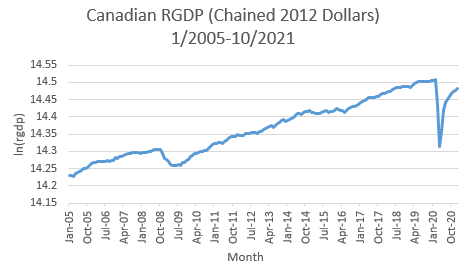
\includegraphics[scale=.48]{RGDP_COVID}
\end{figure}
\end{column}
\begin{column}{0.5\linewidth}
\begin{figure}
\centering
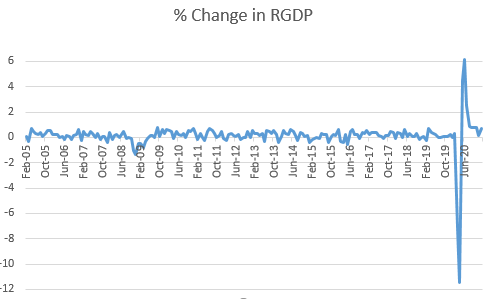
\includegraphics[scale=.4]{P_RGDP_COVID}
\end{figure}
\end{column}
\end{columns}
\end{frame}

\begin{frame}
\frametitle{\: \: \: RGDP-- Cycle}
\toplinemedium
\begin{figure}
\centering
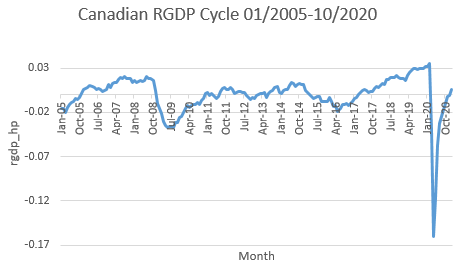
\includegraphics[scale=.67]{RGDP_COVID_cycle}
\end{figure}
\end{frame}


\begin{frame}
\frametitle{\: \: \: Employment in Canada (Total Hours Worked)}
\toplinexlarge
\begin{columns}
\begin{column}{0.5\linewidth}
\begin{figure}
\centering
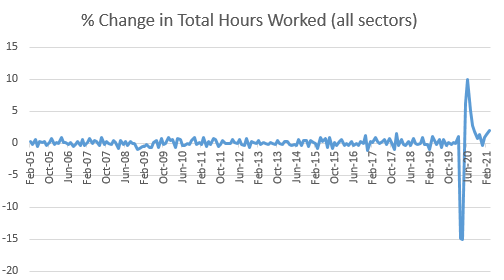
\includegraphics[scale=.43]{employment_alls_canada}
\end{figure}
\end{column}
\begin{column}{0.5\linewidth}
\begin{figure}
\centering
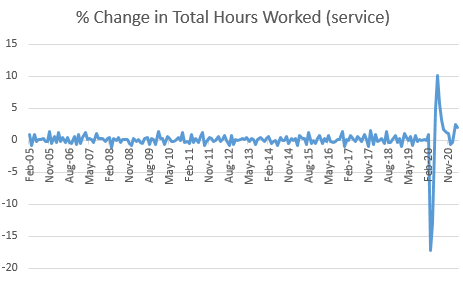
\includegraphics[scale=.43]{employment_s_canada}
\end{figure}
\end{column}
\end{columns}
\end{frame}

\begin{frame}
\frametitle{\: \: \: International Covid Shock}
\toplinelarge
\begin{figure}
\centering
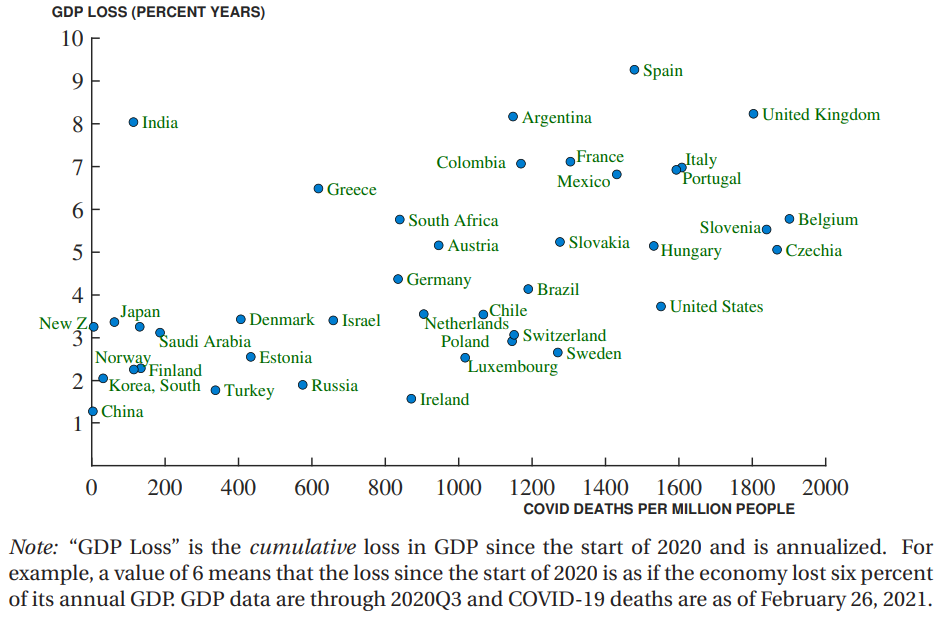
\includegraphics[scale=.4]{international_covid}
\end{figure}
\end{frame}

\begin{frame}
\frametitle{\: \: \: COVID Recession}
\toplinelarge
\begin{itemize}
\item Through the lens of our model, the COVID Recession is hard to analyse because:
\begin{itemize}
\vspace{0.1in}
\item Multiple Shocks to the economy (supply-side and demand-side)
\vspace{0.1in}
\item (Short-run???) shocks to production capacity 
\begin{itemize}
\vspace{0.1in}
\item Our framework allows for either short-run supply shocks to the firm's price setting behaviour (cost-push shocks) or long-run shocks to the production capacity. 
\vspace{0.1in}
\item Consensus is that it affected $\overline{Y}$, which affected demand parameters in the long-run with the short-run adjusting right away (did not see any deflation pressure --- unlike overshooting in the IS-MP model)
\vspace{0.1in}
\item As we recover, agents are failing to see that this is a more permanent effect on $\overline{Y}$, which is why we are currently seeing short-run overshooting.
\vspace{0.1in} 
\item In addition, we are experiencing a cost-push shock due to the war in Ukraine.  
\end{itemize}
\end{itemize}
\end{itemize}
\end{frame}

\section{International transmission of monetary policy}

\begin{frame}
\frametitle{\: \: \: Exchange Rate}
\toplinemedium
\begin{itemize}
\item The Real exchange can be expressed as follow:
\begin{eqnarray*}
RER=E_{C\$/U\$} \frac{P_{U\$}}{P_{C\$}}
\end{eqnarray*}
\vspace{0.11in}
\item Assuming no transportation costs the exchange rate in the long-run is given by the law of one price:
\begin{eqnarray*}
E_{C\$/U\$}=\frac{P_{C\$}}{P_{U\$}}
\end{eqnarray*}
\item In the short run, exchange rates are set by demand for currency, for instance:
\begin{eqnarray*}
\uparrow i^{US} \Rightarrow \uparrow E  \: \: \: \text{    (i.e. Canadian Dollar depreciates)}
\end{eqnarray*}
\item With sticky prices: $\uparrow E \Rightarrow \uparrow RER$
\end{itemize}
\end{frame}

\begin{frame}
\frametitle{\: \: \: Transmission of Monetary policy}
\toplinelarge
\begin{itemize}
\item An change in nominal rates in the US has consequence for the Canadian Economy:
\begin{eqnarray*}
\uparrow i^{US} \Rightarrow \uparrow E \Rightarrow \uparrow RER \Rightarrow \uparrow EX, \downarrow IM
\end{eqnarray*}
\item This has an effect on the expenditure which results in an increase in output.
\begin{itemize}
\vspace{0.11in}
\item This effect is \textbf{similar} to a positive demand shock in our IS-MP and AS-AD model, we will formally study this effect in our SR models next class.
\end{itemize}
\end{itemize}
\end{frame}

\begin{frame}
\frametitle{\: \: \: Transmission of Monetary policy}
\toplinelarge
\begin{itemize}
\item Impact of a change in nominal rates for the Canadian Economy:
\begin{eqnarray*}
\begin{array}{l}
\uparrow i^{US} \Rightarrow \uparrow R^{US} \Rightarrow \uparrow E_{C\$/U\$} \Rightarrow \uparrow RER \Rightarrow \uparrow EX, \downarrow IM \\
\uparrow i^{CA} \Rightarrow \uparrow R^{CA} \Rightarrow \downarrow E_{C\$/U\$} \Rightarrow \downarrow RER \Rightarrow \downarrow EX, \uparrow IM
\end{array}
\end{eqnarray*}
\item To capture this effect, we write the net exports as: $NX=a_{NX}-b_{NX} (R_t-R_t^{US})$
\vspace{0.11in}
\item This results in the following IS curve:
\begin{eqnarray*}
\widetilde{Y}_t=\frac{1}{(1-bc)}\: [\overline{a}-(\overline{b}_i+\overline{b}_{NX}) \: (R_t-\overline{r})]-1
\end{eqnarray*}
\begin{itemize}
\item where $\overline{a}=\frac{a_c+a_i-b_i \: \overline{r}+G+a_{NX}-b_{NX}\: (\overline{r}-R^{US}_t)}{\overline{Y}}$
\end{itemize}
\end{itemize}
\end{frame}

\begin{frame}
\frametitle{\: \: \: Transmission of Monetary policy}
\toplinelarge
\begin{itemize}
\item The effect of domestic monetary policy is similar to before, but amplified. E.g. $\uparrow R_t$: 
\begin{figure}
\centering
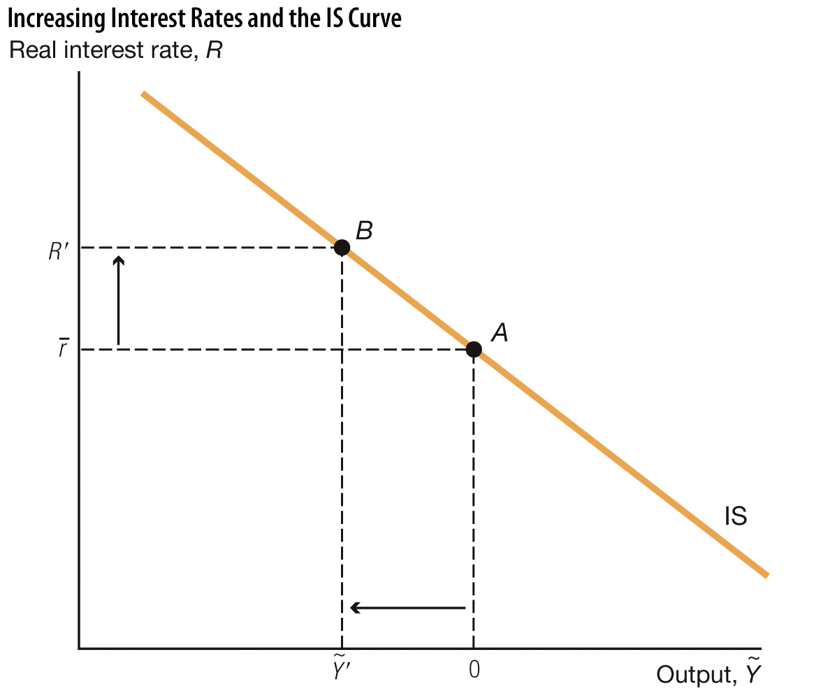
\includegraphics[scale=.3]{monetary_policy}
\end{figure}
\end{itemize}
\end{frame}

\begin{frame}
\frametitle{\: \: \: Transmission of Monetary policy}
\toplinelarge
\begin{itemize}
\item The effect of foreign monetary policy is like a demand shock. E.g. one time increase in $R_t^{US}$:
\begin{eqnarray*} 
\uparrow R^{US}_t \Rightarrow \uparrow \overline{a} 
\end{eqnarray*}
\begin{figure}
\centering
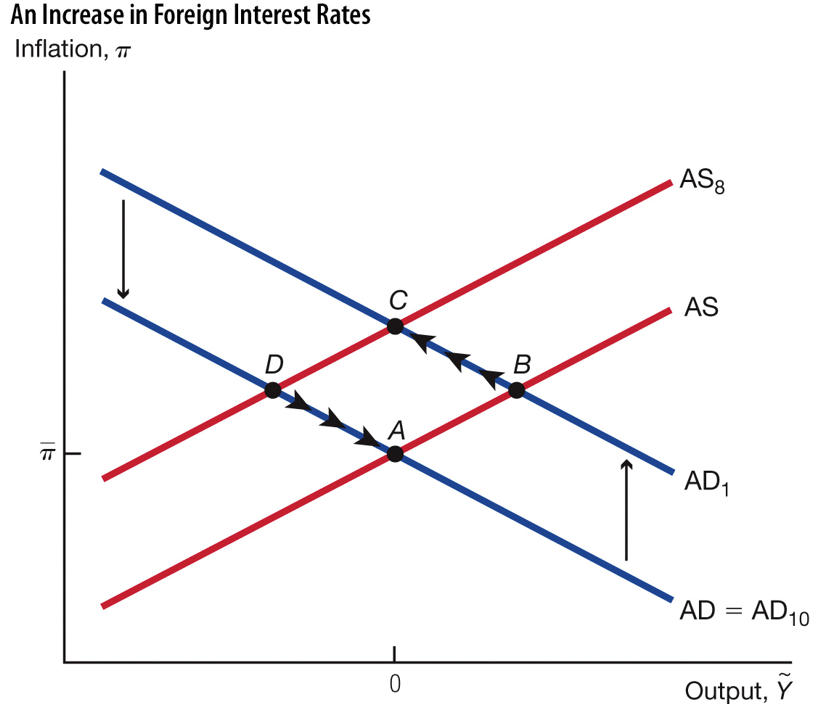
\includegraphics[scale=.3]{foreign_monetary_policy}
\end{figure}
\end{itemize}
\end{frame}

\section{Conclusion}

\begin{frame}
\frametitle{\: \: \: Measuring Aggregate Economic Activity}
\toplinexlarge
In this class, we study how economists measure aggregate economy activity.
\begin{itemize} 
\vspace{.11in}
\item In particular, we studied
\begin{enumerate}
\vspace{.11in}
\item different approaches to measure the value of output (expenditure, income and value added approach) 
\vspace{.11in}
\item how to compare economic activity across time (price indexes):
\vspace{.11in}
\begin{itemize}
\item Chain-Weighting Approach to measure changes in real GDP over the long-run
\end{itemize}
\vspace{.11in}
\item how to compare economic activity across countries:
\vspace{.11in}
\begin{itemize}
\item using PPP-exchange rates
\end{itemize}
\end{enumerate}
\end{itemize}
\end{frame}

\begin{frame}
\frametitle{\: \: \: Long-Run Economic Growth}
\toplinelarge
\begin{itemize}
\item We  also studied the determinants of long-run growth:
\begin{enumerate}
\vspace{.11in}
\item Basic facts about long-run growth across countries
\vspace{.11in}
\item Disaggregate cross-country differences in output per-capita into differences in inputs of an aggregate production function:
\begin{itemize}
\vspace{.11in}
\item $Y=A \:  K^{1/3} \: L^{2/3}$
\end{itemize}
\vspace{.11in}
\item Study two important long-run growth models with very different implications for long-run growth:
\begin{itemize}
\vspace{.11in}
\item Solow Growth Model
\vspace{.11in}
\item Romer Growth Model (Economics of Ideas)  
\end{itemize}
\vspace{.11in}
\end{enumerate}
\item , and the long-run relation between money growth and inflation 
\end{itemize}
\end{frame}

\begin{frame}
\frametitle{\: \: \: Short-Run Economic Fluctuations}
\toplinelarge
\begin{itemize}
\vspace{.11in}
\item Lastly, we studied the determinants of short-run economic fluctuations:
\begin{enumerate}
\vspace{.11in}
\item Basic facts about short-run deviations from potential output
\vspace{.11in}
\item Shocks to the economy, inflation and government monetary policy (IS-MP model as well as standard and non-standard monetary policy instruments)
\vspace{.11in}
\item The central macroeconomics model of short-run economic fluctuations (AS-AD model) with an application to the Great Recession, Covid Crisis and international transmission of monetary policy
\end{enumerate}
\end{itemize}  
\end{frame}

\end{document}